\documentclass[12pt]{article}

\usepackage[margin=3cm]{geometry}
\usepackage{graphicx}
\usepackage{pdfpages}
\usepackage{minted}

\author{Pablo Vargas Bermúdez}

\begin{document}
\pagestyle{empty}
\includepdf[pages=-]{Portada2}

\section*{Planteamiento}

Una vez realizada la tarea \#9 modifica tu programa para que permita
crear en el JFrame una Jtable donde puedas desplegar la información de
la consulta, recuerda crear un JSlider por si se obtienen muchos datos
de la consulta.  Aqui te muestro un ejemplo donde se agregan unos
botones para poder interactuar con la BD:

\begin{center}
  \includegraphics[width=.5\textwidth]{figures/example1.png}
  \includegraphics[width=.5\textwidth]{figures/example2.png}
\end{center}


Envía un archivo PDF que contenga una hoja de presentación, la
descripción de la tarea, el código fuente de la solución y las
capturas de pantalla de las bases de datos que realizaste, mostrando
la información almacenada en las tablas que son consultadas, anexa
también las pantallas necesarias donde muestres el correcto
funcionamiento del programa funcionamiento.

\textbf{NOTA:} No es conectarse a cualquier base de datos, es a la que viene en
el tutorial y la descrita en el PDF de la liga anterior. Puedes usar
cualquier manejador de BD que tengas disponible, no necesariamente
Derby

\section*{Código}

\subsection*{Conexión}
\inputminted{Java}{DataBase.java}
\subsection*{Gui}
\inputminted{Java}{Gui.java}
\subsection*{Prueba}
\inputminted{Java}{PruebaDataBase.java}

\pagebreak
\section*{Bases de Datos}
\subsection*{Amigos}
\begin{figure}[ht]
  \centering
  \includegraphics[width=\textwidth]{figures/tabla.png}
  \caption{Tabla COLLEAGUES}
\end{figure}
\subsection*{Test}
\begin{figure}[ht]
  \centering
  \includegraphics[width=.6\textwidth]{figures/tabla2.png}
  \caption{Tabla testData}
\end{figure}

\pagebreak
\section*{Ejecución}
\begin{figure}[ht]
  \centering
  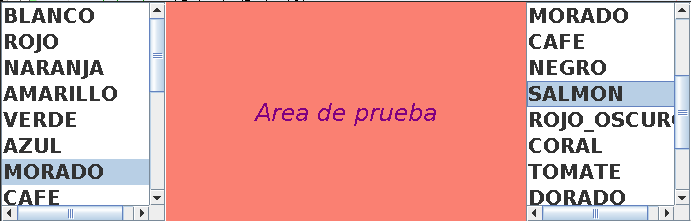
\includegraphics[width=\textwidth]{figures/run1.png}
  \caption{Primera prueba}
\end{figure}

\begin{figure}[ht]
  \centering
  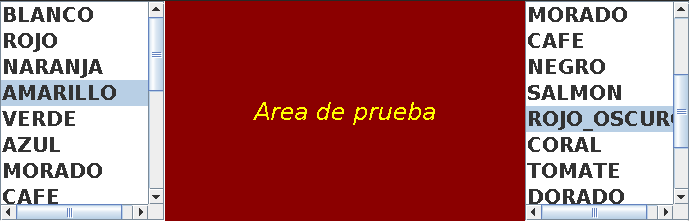
\includegraphics[width=\textwidth]{figures/run2.png}
  \caption{Segunda prueba}
\end{figure}

\begin{figure}[ht]
  \centering
  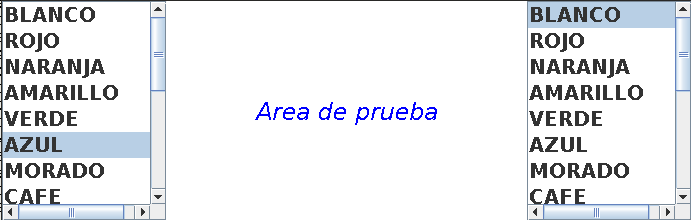
\includegraphics[width=\textwidth]{figures/run3.png}
  \caption{Tercera prueba}
\end{figure}

\begin{figure}[ht]
  \centering
  \includegraphics[width=\textwidth]{figures/run4-1.png}
  \caption{Cuarta prueba, primer prompt}
\end{figure}

\begin{figure}[ht]
  \centering
  \includegraphics[width=\textwidth]{figures/run4-2.png}
  \caption{Cuarta prueba, sedundo prompt}
\end{figure}

\begin{figure}[ht]
  \centering
  \includegraphics[width=\textwidth]{figures/run5.png}
  \caption{Quinta prueba, otra BD ``test''}
\end{figure}


\end{document}